\documentclass{standalone}
\usepackage{tikz}
\usepackage{ctex,siunitx}
\setCJKmainfont{Noto Serif CJK SC}
\usepackage{tkz-euclide}
\usepackage{amsmath}
\usetikzlibrary{patterns, calc,3d}
\usetikzlibrary {decorations.pathmorphing,decorations.pathreplacing,decorations.shapes,}
\begin{document}
\small
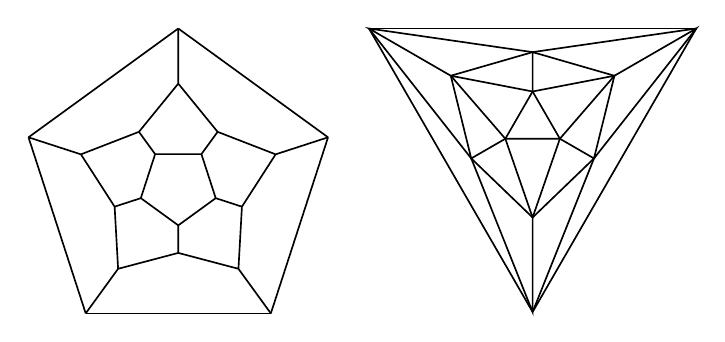
\begin{tikzpicture}[>=latex,scale=1.0,semithick]
  \foreach \x in {18,90,162,234,306}
  {
    \draw(\x:2)--(\x+72:2);
    \draw(\x:2)--(\x:1.3)--(\x+36:0.85)--(\x+36:0.5)--(\x+108:0.5)(\x:1.3)--(\x-36:0.85);
  }
  \begin{scope}[xshift=4.5cm,yshift=0.8cm]
    \foreach \x in {30,150,270}
    {
      \draw(\x:2.4)--(\x+120:2.4);
      \draw(\x:2.4)--(\x+60:0.9)--(\x+120:1.2)--(\x+180:0.9)--(\x+180:0.4)--(\x+300:0.4)--(\x:1.2)--(\x+60:0.4);
      \draw(\x:1.2)--(\x:2.4)--(\x-60:0.9);
    }
  \end{scope}
\end{tikzpicture}
\end{document}